\section{Fish biomass response to ENSO variality}

This section describes the synchronous response of the epipelagic community simulated by the model to ENSO variability in the tropical Pacific. To do so, we focus on the 1997/98 El Niño event because (1) it is the strongest El Niño event on records (\cite{santosoDefiningCharacteristicsENSO2017}) and (2) the ocean response to this specific event has been extensively described and analyzed, in terms of physics  (e.g. \cite{mcphadenGenesisEvolution1997981999, vialardModelStudyOceanic2001, lengaigneOceanResponseMarch2002}, biogeochemistry \citep{chavezBiologicalChemicalResponse1999, gierachBiologicalResponse19972012} and ecosystems (e.g. \cite{leaObservationsFishesAssociated2000, glynnCoralBleachingMortality2001,arcosJackMackerelFishery2001})

Figure \ref{fig:mean_ond97_ape} displays the mean biomass density over the 1958-2018 period (left column) and the biomass density anomalies averaged over the 97 October, November and December (OND) months, when the El Nino signal is at its maximum.

\begin{figure}
	\centering
	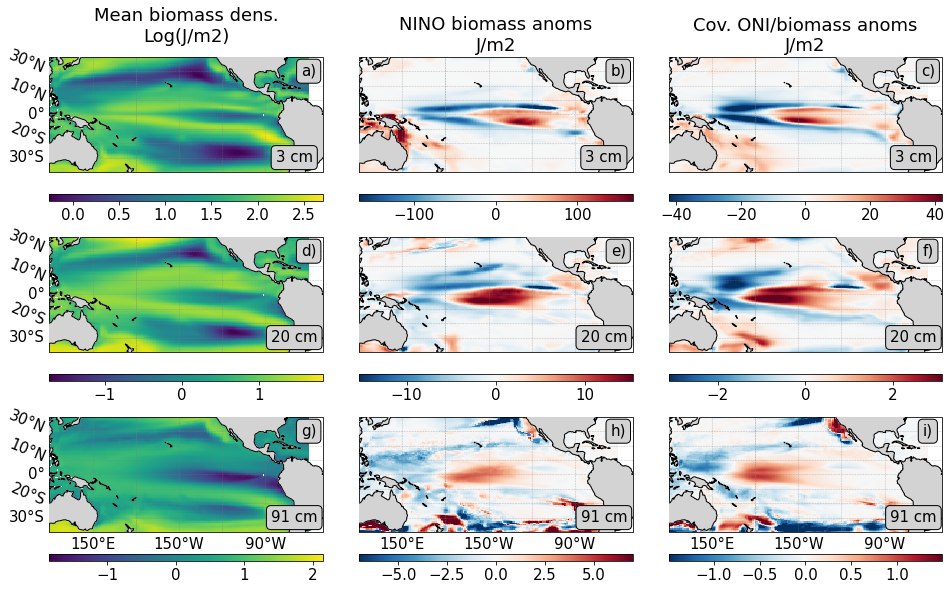
\includegraphics[scale=0.4]{figs/map_mean_anom_OND_97.png}	
	\caption{Mean fish biomass (left column, log-scale), OND-97 anomalies (middle column) and covariance of fish biomass anomalies with the ONI index (right column) for small (upper line), intermediate (middle line) and large sizes (lower line).}	
	\label{fig:mean_ond97_ape}
\end{figure}

For small sizes (Figure \ref{fig:mean_ond97_ape}a), the mean fish biomass is concentrated at around 10° S and 10°N in the central Pacific and close to the equator in the western Pacific. High biomass concentration is also found east of 90° W, off the coasts of Chile. As size increases, the equatorial "blue spot" extends meridionally and to the west. This pattern is mostly driven by the active and passive advection of fishes in the Apecosm model. Without advection, the biomass will be concentrated at the equator, where the plankton concentration is the maximum.

During the 97 El Nino, small epipelagics show negative anomalies in the Western Equatorial Pacific and positive anomalies in the Central Equatorial Pacific. This pattern can be interpreted as an eastern displacement of the mean biomass in the Western Pacific. Similar dipolar patterns are also obtained for intermediate and large sizes, but the anomalies shift westward as size increases. This can be interpreted, as for small sizes, by a westward shift of fish biomass during positive El Niño phases.

These anomalies are very similar to the covariance maps computed between the monthly ONI index and the monthly fish biomass anomalies over the 1958-2018 period (right column of Fig\ref{fig:mean_ond97_ape}), although they are westward shifted and have lower amplitudes than OND-97 anomalies. This is due to the fact that covariance anomalies include El Nino events with different characteristics (Eastern and Central Pacific El Nino, \warn{ref})  and La Nina events, whose characteristics are not opposite to El Nino's ones (\warn{ref}). However, the general agreement between the covariance maps and the OND-97 anomalies suggest that overall, the mechanisms associated with these patterns are likely to be the same.

Figure \ref{fig:profiles} shows the mean equatorial profiles for temperature, zonal velocity, low-trophic level concentration and fish-biomass (contour lines) and the OND-97 anomalies. Temperature shows a deep thermocline in the western Pacific and a shallow one in the east. The anomalies are consistent with a flattening of the thermocline. The structure of the Equatorial Undercurrent is well visible on the zonal velocity profile. During the 97 El Nino, it strongly weakens and strong positive anomalies occur near the surface. The mean low-trophic level concentrations are maximum close to the surface in the eastern Pacific. During the 97 El Nino, negative anomalies superimposes on top of the mean, hence indicating a reduction of plankton concentration, due to the weakening of the upwelling and the associated reduction in nutriments.

Mean profiles of fish biomass show that biomass in the western Pacific is maximum at 50m depth, while in the eastern Pacific, it remains very close to the surface. Small sizes extend further east than large ones, as visible in Fig.\ref{fig:mean_ond97_ape}. During the 97 El Nino, fish biomass shows an increase in the eastern Pacific and a general decrease in the west. However,  the latter is not homogeneous on the vertical, since positive anomalies are located at around 50m in the east. These positive anomalies are more visible for intermediate and large sizes and are induced by a tightening of the vertical habitat and in turn of the vertical distribution of fish biomass.


\begin{figure}
	\centering
	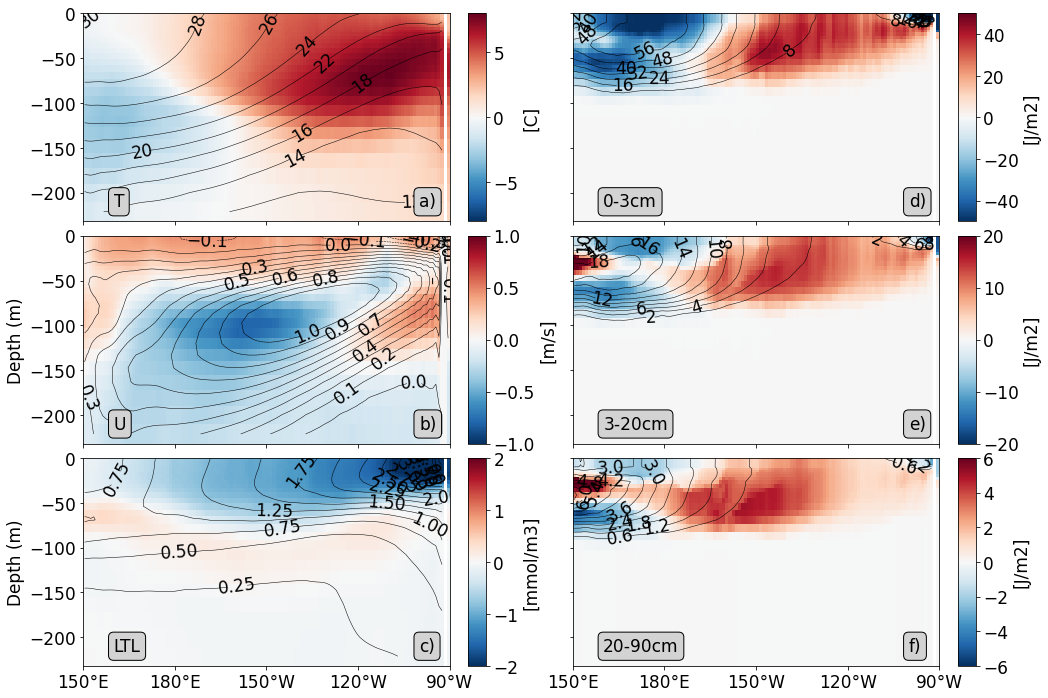
\includegraphics[scale=0.4]{figs/forage_mean_ond97.png}	
	\caption{Pacific equatorial profiles of temperature (a), zonal velocity (b), low-trophic concentration (c) and fish biomass (d for small, e for intermediate and f for large sizes). Mean are represented as black contour lines and El Nino anomalies are represented in colors.}	
	\label{fig:profiles}
\end{figure}

\begin{figure}
	\centering
	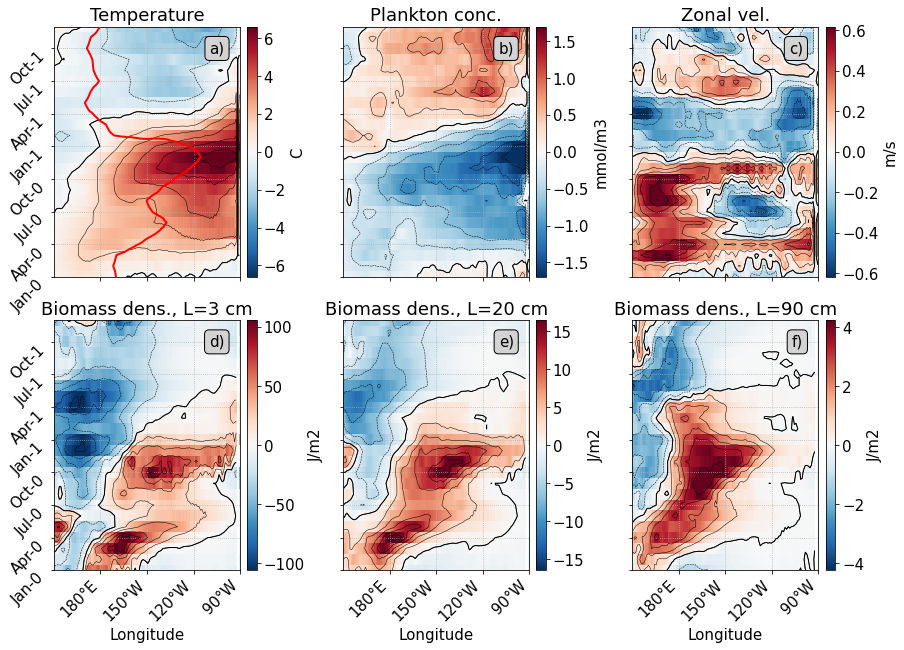
\includegraphics[scale=0.4]{plot_all_hovmoller_phys_oope.png}	
	\caption{Hovmoller diagrams of equatorial temperature (a), low-trophic level concentrations (b), zonal velocity (c) and fish biomass anomalies (3cm, 20cm and 90 cm in d, e, f, respectively).}	
	\label{fig:hov_nemo_ape}
\end{figure}

Figures \ref{fig:hov_nemo_ape}a, \ref{fig:hov_nemo_ape}b, \ref{fig:hov_nemo_ape}c display equatorial hovmüller diagrams of the temperature, chlorophyll and zonal currents anomalies averaged over the top 50m simulated by the ocean model during the 1997/1999 period. In agreement with observations (not shown; see \cite{lengaigneOceanResponseMarch2002}), the warming signal associated with the 1997 El Niño initiates in early spring over the central and eastern equatorial Pacific, peaks by the end of the calendar year in the eastern Pacific to quickly recede and switches La Niña conditions the following spring (Figure \ref{fig:hov_nemo_ape}a). The El Niño warming period is accompanied by strong surface eastward anomalous currents (Figure \ref{fig:hov_nemo_ape}c) promoted by anomalous westerly winds and contributing to central Pacific warming and eastward shift of the warm-pool towards the eastern equatorial Pacific. These current anomalies reverse during La Niña. Simulated plankton concentration anomalies tend to mirror temperature anomalies, with a strong decline during El Niño and an enhanced bloom during La Niña (Figure \ref{fig:hov_nemo_ape}.b). 

The same analysis is then performed for epipelagic biomass for the three targeted size classes (Fig\ref{fig:hov_nemo_ape}d, Fig\ref{fig:hov_nemo_ape}e and Fig\ref{fig:hov_nemo_ape}f), which share some common features: positive biomass anomalies for the three communities appear near the dateline in early spring and propagate eastward towards the central Pacific until the end of summer. Another positive patch then develops in the central Pacific in fall and quickly recedes in winter. These positive anomalies in the central and eastern Pacific  are associated with negative biomass anomalies in the western Pacific during the 1997/98 El Niño. These negative anomalies persist after the El Niño demise and during the following La Niña event but remain restricted to the western Pacific. While sharing similarities, the response of larger epipelagic fishes is generally shifted westward compared to smaller ones.

In order to determine the mechanisms behind the pattern of equatorial fish biomass anomalies during the 97 El Nino, equatorial fish biomass anomalies has been reconstructed for the different processes (growth, predation, advection and diffusion) separately by integrating, over time, equation \ref{eq:apecosm_trend}. The resulting Hovmoller diagrams are presented for the three size classes in Fig\ref{fig:hov_ape_trends_3}, 
Fig\ref{fig:hov_ape_trends_20} and Fig\ref{fig:hov_ape_trends_90}.

\begin{figure}
	\centering
	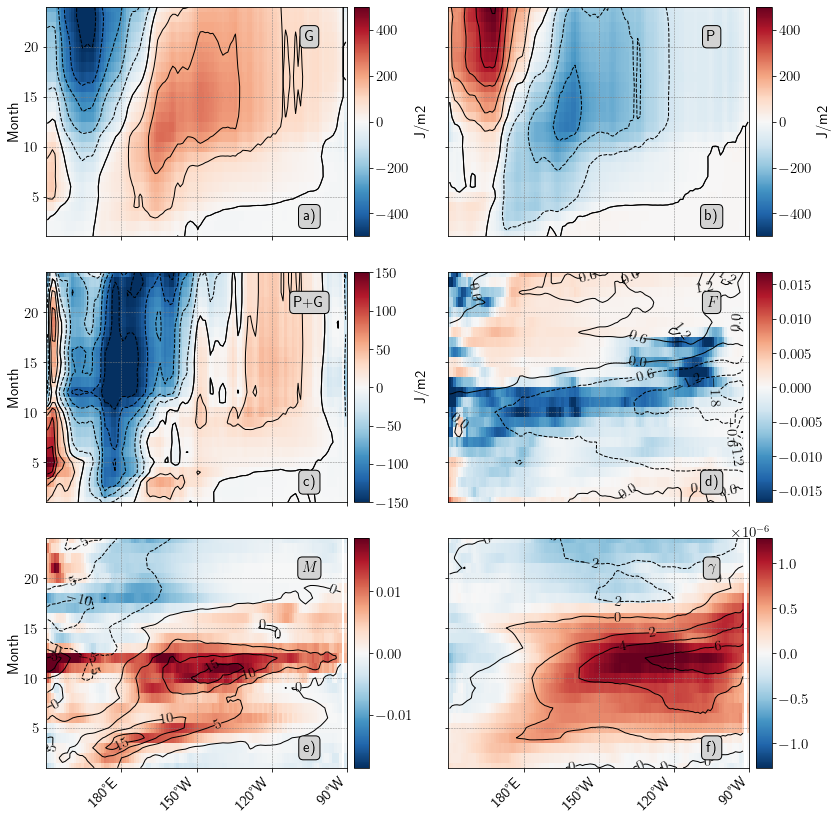
\includegraphics[scale=0.4]{figs/hov_compo_l_3.png}	
	\caption{Hovmoller diagrams of equatorial small fish biomass anomalies induced by predation mortality (P, first line), growth (G, second line), growth + predation (P+G, third line) and movements (advection and diffusion, A+D, bottom line).}	
	\label{fig:hov_ape_trends_3}
\end{figure}

\begin{figure}
	\centering
	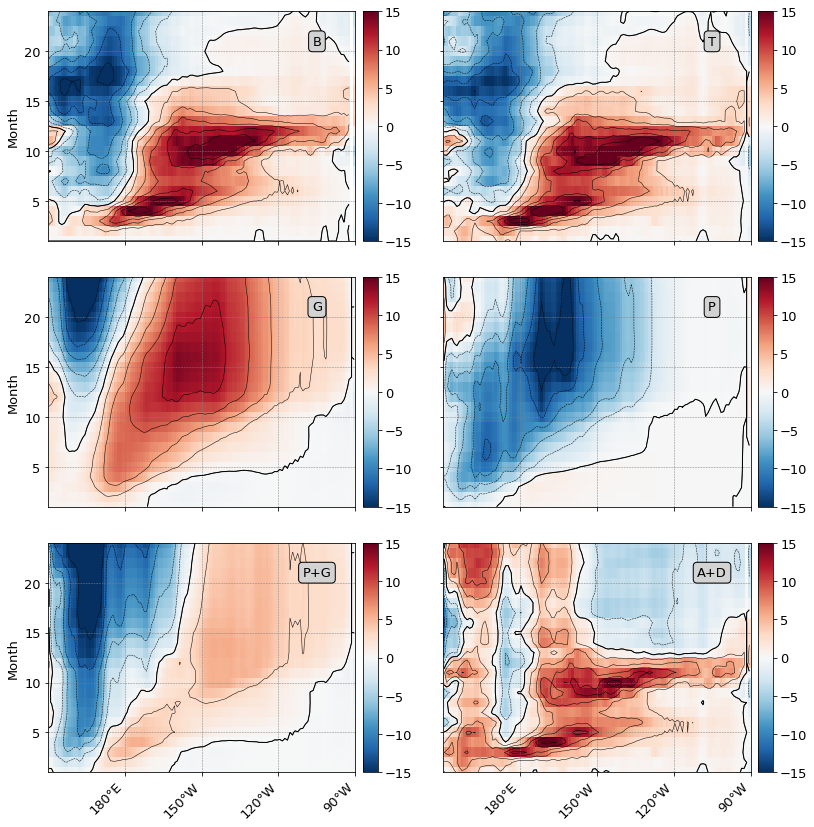
\includegraphics[scale=0.4]{figs/hov_compo_l_20.png}	
	\caption{Hovmoller diagrams of equatorial intermediate fish biomass anomalies induced by predation mortality (P, first line), growth (G, second line), growth + predation (P+G, third line) and movements (advection and diffusion, A+D, bottom line)}	
	\label{fig:hov_ape_trends_20}
\end{figure}

\begin{figure}
	\centering
	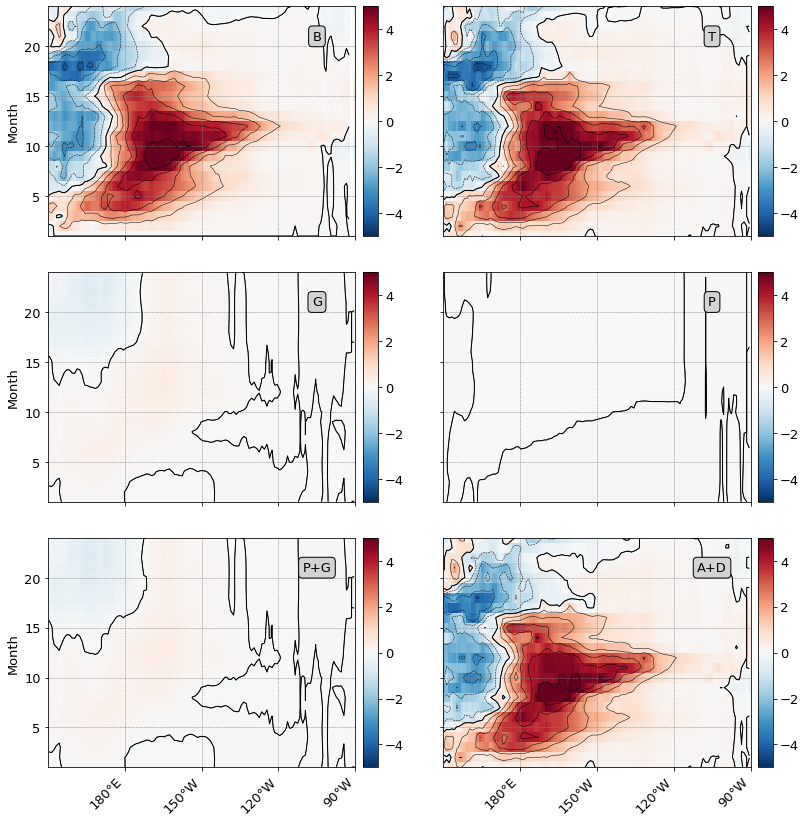
\includegraphics[scale=0.4]{figs/hov_compo_l_90.png}	
	\caption{Hovmoller diagrams of equatorial large fish biomass anomalies induced by predation mortality (P, first line), growth (G, second line), growth + predation (P+G, third line) and movements (advection and diffusion, A+D, bottom line)}	
	\label{fig:hov_ape_trends_90}
\end{figure}


Predation and growth show opposite contributions to changes in small fish biomass (Fig.\ref{fig:hov_ape_trends_3}a and Fig.\ref{fig:hov_ape_trends_3}.b), which are around 3 times larger than the biomass anomalies (Fig. \ref{fig:hov_ape_trends_3}d), implying that at first order these anomalies balance each other. In early 1997, growth induces an increase in the central Pacific (between dateline and 180W), while predation induces a decrease. Starting in 1997-10, these relative contributions to fish biomass anomalies extend to the east, and opposite variations appear in the western Pacific. Interestingly, the anomalies induced by growth are westward shifted and start later than the temperature increase induced by the onset of El Nino conditions. The pattern obtained by summing these two contributions (Fig.\ref{fig:hov_ape_trends_3}.c) is a negative anomaly centered around the dateline and extending from 1997-01 to 1998-12, with the strongest anomalies in early 1998. Advection and diffusion account for an increase in fish biomass from 1997-01 to 1998-12 along a longitudinal band centered on the dateline, which compensates the negative anomalies induced by the combination of growth and predation. Fish movements also induces an increase of fish biomass between 150W and 120W that starts around 1997-10, which is also visible in the fish biomass anomalies (Fig. \ref{fig:hov_nemo_ape}d).

Regarding intermediate size-classes, predation accounts for an intermediate reduction of fish biomass in the eastern Pacific and a strong one in the central Pacific (Fig.\ref{fig:hov_ape_trends_20}e), which reaches its maximum in 1998-04. This biomass reduction due to predation is similar to that of small sizes but westward shifted. Looking at the biomass  changes induced by growth (Fig.\ref{fig:hov_ape_trends_20}f) , we notice a strong increase in the western Pacific, which peaks in 1997-04, and a late increase  in the eastern Pacific. The latter is very similar to the one observed for small sizes, hence indicating similar causes, presumably an greater growth rate due to warmer temperatures. Finally, the contributions of fish movements induce an increase of fish biomass in the west, which compensates the reduction of fish biomass induced by predation. It also shows two distinct increases of fish biomass, one around 1997-04 in the central Pacific and one in 1997-10 in the western Pacific. These increases are visible in the fish biomass anomalies (Fig.\ref{fig:hov_nemo_ape}e), which suggest a dominance of advective and diffusive processes.

For large sizes (Fig.\ref{fig:hov_ape_trends_20}), predation and growth processes are very similar. They are both associated with positive anomalies west of the dateline, and negative anomalies between the dateline and 150W. However, these anomalies do not seem to change much between 1997-01 and 1998-12 and therefore cannot explain the large fish biomass anomalies depicted in Fig.\ref{fig:hov_nemo_ape}f. On the other hand, the fish biomass anomalies induced by advection and diffusion perfectly match the simulated fish biomass anomalies. \warn(Specify if diffusion/advection, specify if active or passive). Therefore, on interannual time-scales, fish biomass for large sizes is not driven by biological processes but by physical ones.

%The patterns of the functional response and growth rates are very different for small sizes (figures YYY.a and YYY.d). The former shows negative anomalies on the central Pacific during the onset of El Nino conditions, presumably due to the concomitant reduction of plankton concentration (figure YYY.b). Interestingly, no anomalies are found in the eastern basin, due to compensating effects of warming temperatures and reduced plankton concentrations. The growth rate shows a pattern that is very similar to the temperature anomalies (Fig. XXX.a), indicating the dominance of temperature on the growth rate. The mortality rate (Fig. YYY.g) shows a pattern that is consistent with the increased biomass of intermediate epipelagics (XXX.b), which predate on small ones.  Besides, growth rate anomalies superimpose well on the small biomass anomalies (black contours in Fig. YYY.d), hence suggesting that the increased biomass during the El Nino conditions is triggered by enhanced growth associated with warmer temperature, despite a dampening effect of increased mortality rates.
%For intermediate sizes, the functional response and the growth rate show very similar anomalies, hence suggesting that they both are driven by the same factors. Both show positive anomalies during the onset of El Nino between 200E and 250E, presumably induced by the temperature warming that favours both the growth and search rates. Then negative anomalies occur, which are westward shifted relative to the positive ones. These negative anomalies are likely induced by the cooling associated with the La Nina conditions reinforced by the reduced small fish biomass that appears near 200E, as shown in Fig. XXX.d. Mortality rates anomalies are consistent with the increase of large fish biomass (Fig. XXX.f). Comparing the different fields, we can suggest that the increased fish biomass that appears on the central Pacific in early 1997 is first dominated by advective processes, which returns a similar pattern (fig YYY.k). Then, during the El Nino peak, the increased biomass of intermediate fish is driven by both an increased growth rate and an increased functional response, which are induced by warmer temperatures and more food available (more small epipelagic fishes, Fig. XXX.d).

%\subsection{Generalisation}
%
%In order to see if ecosystem response to the 97 El Nino event is representative, the covariance between fish biomass anomalies and the ONI index have been computed, following the methodology described in section \ref{sec:cov}. The maps are presented in Fig\ref{fig:ape_cov}.
%
%\begin{figure}
%	\centering
%	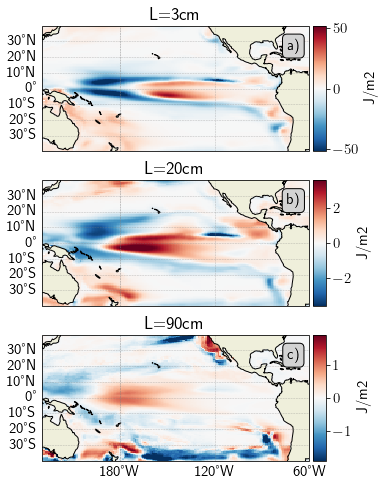
\includegraphics[scale=0.6]{figs/fig7.png}	
%	\caption{Covariance maps between the ONI index and the vertically integrated fish biomass anomalies for small (a), intermediate (b) and large (c) sizes.}	
%	\label{fig:ape_cov}
%\end{figure}
%
%The covariance patterns are very similar to the biomass anomalies depicted in Fig\ref{fig:mean_ond97_ape}, therefore suggesting that the mechanisms described in the above  apply to the general case. However, we note that the covariance patterns are westward shifted compared to the fish biomass anomalies. 
%
%This westward shift might be explained by the fact that when performing covariance anomalies, different El Nino events (Easter Pacific El Nino, Central Pacific El Nino) and La Nina events are considered, which ultimately impacts the global view of fish biomass response to ENSO variability.


%In this section, the interannual response of epipelagics to ENSO variability is investigated using covariance analysis. The left panels of Figure 3. show the yearly mean vertically integrated fish biomass over the entire simulation for the three different size classes. For small sizes (Figure 3a), the fish biomass is concentrated at around 10° S and 10 ° N in the central Pacific and close to the equator in the western Pacific. High biomass concentration is also found east of 90° W, off the coasts of Chile. As size increases, the equatorial "blue spot" extends meridionnally and to the west. This pattern is mostly driven by the active and passive advection of fishes in the Apecosm model (REF). Without advection, the biomass will be concentrated at the equator, where the plankton concentration is the maximum.
%
%Covariance maps between vertically integrated fish biomass and the winter ONI index are shown in the right panels of Figure 3. Small epipelagics show negative anomalies in the Western Equatorial Pacific and positive anomalies in the Central Equatorial Pacific. This pattern can be interpreted as an eastern displacement of the mean biomass in the Western Pacific. Similar dipolar patterns are also obtained for intermediate and large sizes, but the anomalies westward shifted as size increases. This can be interpreted, as for small sizes, by a westward shift of fish biomass during positive El Niño phases. The same results have been obtained when the covariance analysis is performed on monthly anomalies (not shown).